% THIS IS SIGPROC-SP.TEX - VERSION 3.1
% WORKS WITH V3.2SP OF ACM_PROC_ARTICLE-SP.CLS
% APRIL 2009
%
% It is an example file showing how to use the 'acm_proc_article-sp.cls' V3.2SP
% LaTeX2e document class file for Conference Proceedings submissions.
% ----------------------------------------------------------------------------------------------------------------
% This .tex file (and associated .cls V3.2SP) *DOES NOT* produce:
%       1) The Permission Statement
%       2) The Conference (location) Info information
%       3) The Copyright Line with ACM data
%       4) Page numbering
% ---------------------------------------------------------------------------------------------------------------
% It is an example which *does* use the .bib file (from which the .bbl file
% is produced).
% REMEMBER HOWEVER: After having produced the .bbl file,
% and prior to final submission,
% you need to 'insert'  your .bbl file into your source .tex file so as to provide
% ONE 'self-contained' source file.
%
% Questions regarding SIGS should be sent to
% Adrienne Griscti ---> griscti@acm.org
%
% Questions/suggestions regarding the guidelines, .tex and .cls files, etc. to
% Gerald Murray ---> murray@hq.acm.org
%
% For tracking purposes - this is V3.1SP - APRIL 2009\documentclass{acm_proc_article-sp}

\documentclass{sig-alternate}

\usepackage[block=ragged]{biblatex}
\usepackage{listings}
\usepackage{textcomp}
%\usepackage{url}
\bibliography{thinkcs.bib}

\begin{document}
\conferenceinfo{ITiCSE'12,} {July 3--5, 2012, Haifa, Israel.} 
\CopyrightYear{2012} 
\crdata{978-1-4503-1246-2/12/07} 
\clubpenalty=10000 
\widowpenalty = 10000

\title{Analysis of Student Programming Errors in a Large Python Dataset}
%
% You need the command \numberofauthors to handle the 'placement
% and alignment' of the authors beneath the title.
%
% For aesthetic reasons, we recommend 'three authors at a time'
% i.e. three 'name/affiliation blocks' be placed beneath the title.
%
% NOTE: You are NOT restricted in how many 'rows' of
% "name/affiliations" may appear. We just ask that you restrict
% the number of 'columns' to three.
%
% Because of the available 'opening page real-estate'
% we ask you to refrain from putting more than six authors
% (two rows with three columns) beneath the article title.
% More than six makes the first-page appear very cluttered indeed.
%
% Use the \alignauthor commands to handle the names
% and affiliations for an 'aesthetic maximum' of six authors.
% Add names, affiliations, addresses for
% the seventh etc. author(s) as the argument for the
% \additionalauthors command.
% These 'additional authors' will be output/set for you
% without further effort on your part as the last section in
% the body of your article BEFORE References or any Appendices.

\numberofauthors{3} %  in this sample file, there are a *total*
% of EIGHT authors. SIX appear on the 'first-page' (for formatting
% reasons) and the remaining two appear in the \additionalauthors section.
%
\author{
% You can go ahead and credit any number of authors here,
% e.g. one 'row of three' or two rows (consisting of one row of three
% and a second row of one, two or three).
%
% The command \alignauthor (no curly braces needed) should
% precede each author name, affiliation/snail-mail address and
% e-mail address. Additionally, tag each line of
% affiliation/address with \affaddr, and tag the
% e-mail address with \email.
%
% 1st. author
\alignauthor
Brad Miller
       \affaddr{Luther College}\\
       \affaddr{700 College Dr.}\\
       \affaddr{Decorah, IA 52101}\\
       \email{bmiller@luther.edu}
% 2nd. author
\alignauthor
David Ranum
       \affaddr{Luther College}\\
       \affaddr{700 College Dr.}\\
       \affaddr{Decorah, IA 52101}\\
       \email{ranum@luther.edu}
% 2nd. author
\alignauthor
John Doorenbos
       \affaddr{Luther College}\\
       \affaddr{700 College Dr.}\\
       \affaddr{Decorah, IA 52101}\\
       \email{doorjo01@luther.edu} }


\date{30 august 2014}
% Just remember to make sure that the TOTAL number of authors
% is the number that will appear on the first page PLUS the
% number that will appear in the \additionalauthors section.

\maketitle
\begin{abstract}
Very abstract
\end{abstract}

% A category with the (minimum) three required fields
\category{I.7.4}{Computing Methodologies}{Document and Text Processing}{Electronic Publishing}

%\terms{Documentation}
\keywords{CS1, Python, Sphinx, eBook} % NOT required for Proceedings

%\section{Introduction}
\section*{Introduction}



\section*{Related Work}


Gaining a better understanding of how students interact with and react to their programming environment has long been an important part of teaching novice programmers.  Since programming involves learning a programming language and then using it correctly and effectively, aspects of programming language system implementation are often linked to student success.  For example, the role of syntax errors as a cause of frustration and a barrier to learning has been of interest for many years [A,B].  Without syntactic correctness, students cannot move on to more logically based debugging since programs will not execute.  

Although most of these efforts have involved compiler errors from languages such as Java, other languages have also been used as the basis for studying student response to errors.  For example, Marceau et al (M) used a Scheme-based environment to develop a language independent rubric for classifying many types of student errors as a way to understand the effectiveness of error messages.  Since error messages are one of the first points of contact for a student learning to program, one would assume that information they provide is extremely important.  Denny [C] enhanced the error messages by including examples of how the error occurs and possible ideas for what can be done to fix the error.  Interestingly, even with these enhancements, students showed no significant improvement when it came to resolving the error.

In order to study student behavior with respect to resolving errors, it is useful to have comprehensive datasets from students carrying out the same task.  Projects such as BlueJ have allowed researchers to gather large amounts of data pertaining to the behavior of novice programmers [I J].  The BlueJ Blackbox project [K] has begun to collect data related to IDE use and editing history.  This rich dataset is also being made available to other researchers.

Of particular interest for this paper is the notion that Python is considered an excellent language for use in introductory computer science courses [D,E,F,G].  Furthermore, it has even been suggested that it may now be the most popular programming language for introductory teaching [N]. Still, like all programming language environments, Python error messages are not always easy for novice programmers. 

Recently, Miller and Ranum [O,P] have created Runestone Interactive as a new and unique vision for the creation and use of electronic textbooks. The Runestone project provides tools for creating active components and content in the context of an open source authoring system.  In addition, since the courseware is offered online, perpetual data gathering is possible giving rise to the Runestone Data Set.




\section*{The Data Set}

Over the last two years, Runestone Interactive has been gathering information about the websites’ users. Every time a user interacts with the site, a row is added to a table that captures specifics about the event, including the owner of the action; its timestamp, the course the user is associated with, and the event that occurred (i.e. a page load, or the answering of a multiple choice question) along with its result (i.e. whether or not the student answered the multiple choice question correctly). None of the user’s sensitive information is stored in the database. As the database has grown, this information has become more useful for analyzing student activity.   
The online textbook has experienced a huge amount of use by universities, secondary schools, and third party users, causing the database to grow rapidly. After only two years, the database has logged over 17 million actions by students and hobbyists. Universities that use the course include the University of Toronto, the University of Kentucky, and the University of Georgia.
In order to do analysis on the information gathered by the website, it had to be cleaned. There were three main groups that were removed: non-students, corrupt/miscellaneous rows, and outliers. Deciding who was a student, and who was not, was based on many different criteria. It was clear from the beginning that users who only visited to website once shouldn’t be considered students. However, other non-students included all of the course instructors, user IDs that were shared by entire classes of students, and users who didn’t log enough activity to allow for reasonable analysis. 
The corrupt/miscellaneous group of removed data takes out data that includes; pages and interactive elements that don’t appear in the official list provided by the textbook, users that have no username, or courses that are not associated with either of the two analyzed books.  
Outliers were calculated by two different parameters: clicks and duration. The clicks measurement is a count of how many events each user logged on the website, while duration measures how long a user is active on the site. For each parameter, the average and standard deviation are found for all users. Any user that has clicks or duration outside of three standard deviations from the mean is removed as outliers. In order to accurately calculate the outliers, they are found after all database cleaning has taken place. All in all, even after almost half of the database was removed, we were left with 9 million entries in a cleaned dataset ready for analysis. 
In order to provide a level of confidentiality to the websites users, all user and course names have been anonymized. Both registered and unregistered users are assigned an ID number that all of their information is connected to. Courses are also given ID numbers, along with a specification of what the course type is, whether it is a high school course, a college course, or one offered in an informal academic setting.  

While single time users were removed from the dataset because they disrupt the analysis of those students who are using the online textbook as a course, they do provide interesting insight. By finding the pages with the most hits from single time users, we gained an insight into some of the topics students sought  for online help, indicating topics they struggle with. We found the chapters on sorting algorithms and the Stack data structure to be the most common hits by single time users.  Another interesting statistic we looked at was the single time user activity over time. Not surprisingly we saw an overall increase in the website’s activity the longer it was up, but we also found a very uncharacteristic spike in the graph. We found that on Dec 13, 2011 there was a spike in the number of google hits unaffiliated with any courses.  There was almost %250 more hits on that day than any other day in the graph. Eventually we found that on that day a link to the website had been shared on Reddit, causing thousands of new users to explore the site. While this was of no interest to our particular research, it further showed the impacts of social media. 


%!TEX root = thinkcs.tex

\section*{Analysis of Student Errors}

In the summer of 2013 we received a SIGCSE special projects grant to make several enhancements to our interactive textbooks, this included many projects:

\begin{itemize}
	\item A responsive design so the books were easy to read on tablets and phones as well as desktop computers.
	\item Adding answers to the odd numbered homework exercises
	\item Adding discussion areas for homework exercises
	\item Improving the error messages displayed to the students from activecode examples and exercises
\end{itemize}

One question we were particularly interested in exploring in the data set, was the impact of all of these changes to the exercises.  In particular we were intrigued by assertion in \ref{errors} that better error messages don't help students very much.  In our case, we had a lot of control over how error messages were displayed, and we had a year of data where error messages were simply displayed to students in an alert box, and a full year of data where we displayed error messages as shown in Figure~\ref{fig:newmess}.

\begin{figure}[htbp]
	\centering
		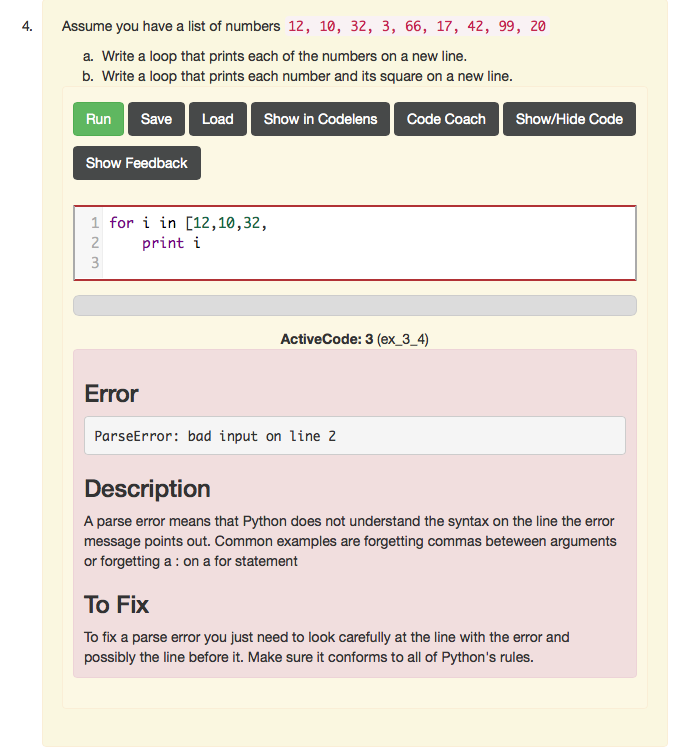
\includegraphics[scale=0.5]{emessage.png}
	\caption{A new style error message}
	\label{fig:newmess}
\end{figure}

As a Python instructor there are many interesting aspects of the exercises to compare from year one to year two.  

\begin{itemize}
	\item How ``efficient'' are students when they do their work?  How many attempts do they make to solve a particular problem?
	\item How often do they simply give up without solving the problem?
	\item What are the most common errors that students encounter?
	\item When students encounter an error how long does it take them to fix that particular error type?
	\item Are certain errors more problematic for students to fix than others?
\end{itemize}

To answer the first question we looked at the total number of times each student attempted the various end of the chapter programming exercises.  We only compared the even numbered questions since we had added the answers to the odd numbered questions in year two.  What we found was that overall from year one to year two the overall average number of attempts to complete and exercise declined by 7.  This of varied by exercise, so we graphed the number of attempts in year two minus the number of attempts in year one.    Figure~\ref{fig:attempts} illustrates the difference on a per question basis. The bars falling below the line illustrate those that took fewer attempts in year two.  You can see that nearly all of the questions took fewer attempts in the second year than the first.

\begin{figure}[htbp]
	\centering
		\includegraphics[scale=1]{errDiffs.png}
	\caption{caption}
	\label{fig:attempts}
\end{figure}

Which exercises took significantly fewer attempts?





\section*{Summary and Future Work}



%\section{References}
\printbibliography
%\bibliographystyle{abbrv}



\end{document}